\begin{justify}
\chapter[Fundamentos Teóricos y Métodos]{Fundamentos Teóricos y Métodos}
\label{ch:marcoteorico}
\section{Marco Teórico}
En este capítulo se introducirán conceptos y problemas que serán abordados durante el desarrollo del proyecto, a través de la recopilación y análisis de información relacionada con el foco central de la investigación, además se explicará cada concepto clave relacionado al proyecto y luego se establecerá la relación de esta materia con el proyecto.

\subsection{ALOHAnet}
El sistema ALOHA, nació con el fin de crear un sistema que se adapte a aquellos escenarios donde las limitaciones de los diseños de redes computacionales implementados bajo conexiones cableadas no se adaptan a las condiciones a las que será expuesto, es decir, situaciones donde son preferibles las comunicaciones sobre la base de la radio frecuencia, por sobre las comunicaciones sobre las conexiones cableadas ~\cite{NORMAN}.\\
La estructura de funcionamiento del sistema ALOHA, consta de un computador central conectado a un canal de comunicaciones por radio frecuencia, donde se poseerán dos bandas de un tamaño de $100KHz$ en las bandas $407.350 MHz$ y $413.475MHz$, una de estas bandas estará destinada a la recepción de información desde los clientes al computador central, y la otra a el envío de información desde el computador central hacia los clientes, donde se genera un método de acceso aleatorio de multiplexación de un gran número de clientes de baja tasa de envío de datos hacia el computador central, donde la comunicación se lleva a cabo por un único canal de comunicaciones por radio.~\cite{NORMAN} Si bien los mensajes desde o hacia la computadora central no se pueden multiplexar, si se pueden utilizar técnicas como la multiplexación del canal y del tiempo, para dividir el canal de comunicaciones desde las consolas hacia la computadora central en un gran número de canales donde cada uno de los clientes usará una de estas subdivisiones del canal, esté activo o no, dado que si se otorgara tiempo de conexión exclusiva a una fracción del número total los clientes activos de la red, este esquema tendría las mismas deficiencias que el diseño de conexión cableada ~\cite{Abdullah}.\\
Como puede apreciarse en la Fig~\ref{aloha:msg}, la estructura de los paquetes de datos que conformarán las trazas de datos en el protocolo ALOHA, constan de un tamaño de a lo más $704 bits$, de los cuales pueden usarse $80$ caracteres de $8 bits$ cada uno (un total máximo de $640 bits$ de payload), $32 bits$ de control y paridad, más 32 bits de identificación. Estos paquetes están diseñados para transmitirse en un tiempo a lo más de $29 ms$ a una tasa de $24000 baudios$(número de símbolos/segundos)~\cite{NORMAN}.\\
\begin{figure}[!ht]
\centering
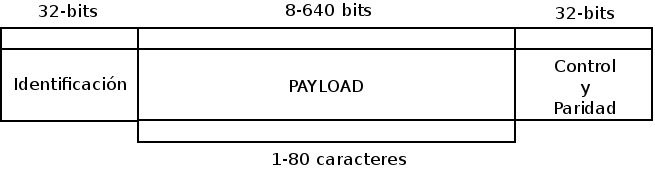
\includegraphics[scale=0.5]{images/alohamsg.png}
\caption{Formato de mensaje de protocolo ALOHA}
\label{aloha:msg}
\end{figure}\\
Con respecto al funcionamiento de este sistema ALOHA, este posee un tipo de conexión asíncrona donde los usuarios activos de una red con este sistema usarán un acceso aleatorio a la red, donde sólo se tomará en cuenta el tiempo donde se comienza el envío de los paquetes de datos y los canales disponibles para la transmisión (en base a la potencia del nodo y la disponibilidad del canal), dado que luego de esperar el doble del tiempo máximo de propagación, en el que  no recibe un paquete ACK (``\textit{Acknowledge}'') que verifique la llegada del paquete enviado. El cliente retransmitirá este paquete periódicamente, hasta recibir un acuse de recibo por su contra parte. Para definir los límites de uso y capacidad del canal, en \cite{NORMAN} se establece que el número máximo de clientes simultáneos en la red es de $324$ clientes, dado que sobre dicho valor, la comunicación se vuelve inestable y con esto, el número promedio de retransmisiones se vuelve ilimitado por lo que satura el canal de comunicaciones~\cite{NORMAN}.\\
Este sistema es de vital importancia para este proyecto de titulo, dado que los dispositivos LoRa basan su comunicación en un sistema ALOHA puro (sistema descrito en esta sección), y ALOHA slotted o ``ALOHA \textit{con espacios}'',donde se agrega una comprobación de canal si está ocupado o no antes de transmitir (``\textit{Listen Before Talk}'')~\cite{Sornin}~\cite{Sornin2}. De esta manera se aumenta el Throughput por fracción de tiempo, por lo que es central el tener este sistema como antecedente al desear simular un comportamiento similar, conocer que destaca a LoRa por sobre ALOHA y para definir que variables se han de agregar a un modelo de ALOHA para que se comporte como LoRa .
\subsection{Spreading Factor}
El acceso dinámico al espectro es una técnica que permite una optimización del uso de los espectros de frecuencia a usar para comunicaciones inalámbricas, donde se expande el espectro de la señal a utilizar para un determinado payload, con el fin de blindar la señal generada por la frecuencia base, por este espectro expandido, lo que protege la señal contra interferencias externas de señales angostas, como también de intercepciones de la señal, dado que el receptor debe conocer la banda base para poder decodificar y demodular la señal de espectro expandido ~\cite{modulation}.\\
Spreading Factor es el nombre utilizado por los desarrolladores de LoRa, para cada frecuencia base que se podrá utilizar como canal de comunicaciones entre los Gateway LoRa y los nodos. Los Spreading Factor, poseen la característica de que al utilizar el Spreading Factor con mayor alcance de transmisión, se sacrifica velocidad de transmisión, por lo que el Spreading Factor con menor alcance ( aproximadamente $2km$ de alcance), transmite a la mayor tasa de bits por segundo (aproximadamente $5470bps$)~\cite{orange}.\\
Adicionalmente los dispositivos LoRa analizan los espectros de frecuencia disponibles, donde luego para el caso particular de LoRa se usa una técnica llamada ``Listen-Before-Talk'' (LBT) la que indica que en vez de probar una conexión y luego evaluar la condición del canal de radio, primero se debe censar y encontrar un canal disponible para de forma posterior iniciar la conexión con él~\cite{modulation}.
\subsection{Dispositivos LoRa}
Los dispositivos LoRa son artefactos para la comunicación inalámbrica de largo alcance, los que fueron diseñados con el fin de generar redes M2M (máquina a máquina) como IoT (Internet de las cosas) para así automatizar tareas de supervisión y censo de datos (usando sensores). Estos datos son distribuidos a través de una topología estrella hacia una puerta de enlace (Gateway), donde el Gateway es el encargado de distribuir los datos hacia el microcomputador o servidor que realizará la conexión con la aplicación deseada.\\
El protocolo usado por estos dispositivos es LoRaWAN, el que permite al Gateway el transmitir configuraciones distribuidas (sincronización de reloj, uso de frecuencia definida, etc.), como también permite adaptar la tasa de envío y el delay de  la transmisión en pro de mejorar la comunicación con el/los nodos~\cite{Sornin}.\\
Los dispositivos clase B que utilizan este protocolo poseen optimizaciones para una mayor duración de la batería gracias a que los dispositivos entran en un modo reposo una vez realizada la subida de datos al servidor, donde el Gateway realiza una sincronización de relojes internos con el nodo, para luego calendarizar el próximo envío de datos~\cite{Sornin}.\\
Con respecto a la estructura del protocolo LoRaWAN, en este proyecto se centrará sobre el funcionamiento de la capa física (MAC) de LoRa. Esta capa posee tres clases principales dependiendo de la complejidad del dispositivo (clase A,B y C), las que definen la cantidad de funcionalidades presentes en el dispositivo.\\
Para el caso de los dispositivos bi-direccionales Clase A (funcionalidad mínima presente en todos los dispositivos)~\cite{Sornin2}, estos dispositivos permiten la comunicación tanto de envío como de recibo de información, pero este espacio de transmisión depende de una pequeña variación aleatoria en el tiempo calendarizado que permite minimizar la cantidad de colisiones en la recepción de paquetes por parte del Gateway (protocolo tipo ALOHA)~\cite{Sornin}. Por otra parte, la obtención de datos desde el servidor a el nodo, debe esperar hasta la ventana de transmisión calendarizada, mientras que el nodo sólo requiere una ventana de bajada para sincronizar su configuración, después de haber transmitido hacia el servidor.\\
Así pues los dispositivos bidireccionales de clase B (Gateway), permiten una mayor capacidad de espacios de recepción (o de conexiones entrantes), y para esto el Gateway transmite una guía de sincronización (con los datos de su reloj interno) para así minimizar la posibilidad de colisiones de paquetes. Además los Gateway son capaces de adaptar entre la tasa de envío de datos y la sensibilidad de la transmisión, para mejorar la calidad del enlace a largas distancias de transmisión. Esta tasa adaptativa de envío de datos (ADR) es implementada en distintos canales que usan distintos espectros de frecuencia (``\textit{Spreading Factor}''), lo que disminuye considerablemente las colisiones, dado que entre Spreading Factors no existen colisiones dado que los espectros de frecuencia poseen la suficiente diferencia.\\
Y en cuanto a los dispositivos de clase C, estos mantienen ventanas de transmisión casi continuas, ya que sólo las cierran al tener que transmitir. Estos dispositivos tienen un mayor consumo de energía en comparación con los dispositivos clase A y B, pero ofrecen la menor latencia en la comunicación servidor-nodo~\cite{Sornin}.\\
En cuanto al protocolo LoRaWAN, este posee una pila de 4 capas, las cuales son: La capa de aplicación, capa MAC, capa PHY y capa RF. Para este proyecto, se trabajará sobre la capa física o PHY ya que el objetivo de la simulación, es imitar el comportamiento físico de los dispositivos LoRa~\cite{Sornin2}.\\
Sobre la motivación por el estudio de los dispositivos LoRa, a causa de poseer una gran diversidad de usos~\cite{use1}~\cite{use2}, son de gran interés para el área de TI, considerando que permiten generar soluciones integrales de redes M2M (Máquina a máquina)/IoT(Internet de las cosas) de forma inalámbrica y a bajo costo en comparación con otras soluciones. Además estos dispositivos tienen la capacidad de transmitir a largas distancias ($2.5 km$ en zonas urbanas densas y $15 km$ en zonas suburbanas), sin necesidad de una infraestructura costosa como es el caso de la tecnologías con una capacidad similar de transmisión como por ejemplo: GPRS, EDGE y LTE. No obstante aún no existen herramientas que permitan el diseño virtual de redes con estos dispositivos con el fin de: probar nuevos usos para esta tecnología, probar rendimientos esperados de una distribución específica, etc.. Bajo este contexto, este proyecto pretende ser un aporte a la comunidad TI en el desarrollo de un modelo de simulación sobre la base del software de simulación de redes OMNET++, el que permitirá replicar el funcionamiento físico de los dispositivos LoRa (Gateway y nodos).
\subsubsection{Formato de Mensaje LoRa}
Si se observa la Fig~\ref{fig:msg}, se puede ver que los mensajes en LoRaWAN poseen una estructura dividida en 4 capas de la misma forma que la pila del protocolo. La primera capa llamada Radio PHY Layer, tiene como objetivo el realizar la conexión de radio frecuencia entre los dispositivos que se disponen a transmitir datos. Por otra parte la capa física está encargada de construir las tramas del mensaje (frame) con el fin de que, la capa de enlace transmita el Payload desde la capa MAC sobre el enlace de radio frecuencia . La capa física (PHY) usa bandas específicas de radio frecuencia dependiendo de la normativa de cada país\cite{Sornin}.\\
\begin{figure}[!ht]
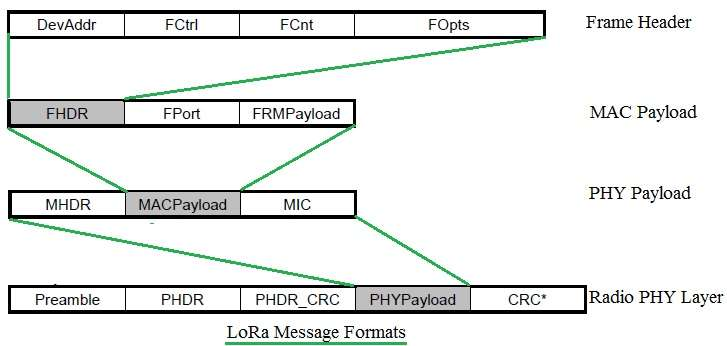
\includegraphics[scale=0.5]{images/LoRa-message-formats}
\caption{Formato de mensaje de protocolo LoRaWAN. Fuente:~\cite{Sornin}}
\label{fig:msg}
\end{figure}
\noindent
Para este proyecto se manipulará el modelo de simulación del protocolo ALOHAnet con el fin de agregar los indicadores de la capa física y de enlace del protocolo al modelo de simulación, esto junto a la modificación de especificaciones de transmisión del enlace de radio frecuencia, a fin de imitar el funcionamiento físico del dispositivo LoRa, y con esto replicar distribuciones y comportamientos esperados de los dispositivos físicos pero de manera virtual.\\
En cuanto a el contenido de cada fragmento de los mensajes enviados por dispositivos LoRa, estos están especificados en las especificaciones técnicas del fabricante, los que son expuestos en la Tabla~\ref{tab:loramsg}~\cite{Sornin}.\\
Los indicadores a usar para el modelo de simulación planeado, son aquellos pertenecientes a la capa RF PHY, a la capa PHY Payload y la capa MAC Payload, sin contar tramas de capas superiores, dado que la herramienta de simulación trabaja en sobre la base de eventos, no analizando paquetes como lo haría un ``\textit{sniffer}'' de red, por lo que algunos campos de información contenida en la cabecera del mensaje es omitida dado este antecedente.
\begin{table}[!ht]
\begin{tabular}{|c|l|}
\hline
Campo de Mensaje LoRa MAC & Descripción \\\hline
MHDR & Cabecera	MAC, longitud de un octeto\\\hline
MAC Payload	& Datos de capa superior\\\hline
MIC	Message Integrity Code & longitud de cuatro octetos\\\hline
FHDR  &	Cabecera de tramas de mensaje\\\hline
FPort	& Campo opcional de puerto de conexión\\\hline
FRMPayload	& Campo opcional de Payload \\&de tramas de mensaje\\\hline
Devaddr	& Dirección de dispositivo\\\hline
FCtrl & Octeto de control de tramas de mensaje\\\hline
FCnt &	Contador de tramas de mensaje,\\& longitud de dos octetos\\\hline
FOpts &	Opciones de trama, usadas para \\&ordenes de transporte\\ & en la capa MAC, longitud de \\&quince octetos\\\hline
\end{tabular}
\caption{Glosario de campos de mensajes LoRa}
\label{tab:loramsg}
\end{table}
\subsection{Diferencias entre LoRaWAN y ALOHAnet}
En relación a la diferencia entre LoRaWAN y ALOHAnet, esta radica en que el protocolo LoRaWAN, si bien posee una implementación del protocolo ALOHA slotted, este protocolo es capaz de mediante comandos MAC el colocar en modo reposo a los clientes que no necesiten mandar paquetes y calendarizar su próxima entrega de información, donde gracias a una sincronización de relojes entre el cliente y la puerta de enlace ( o concentrador LoRa), es posible generar un ahorro de consumo de energía considerable en los nodos, dando así una mayor autonomía a los dispositivos. Junto con esto, LoRaWAN posee una optimización de los usos de los canales de transmisión, ya que a diferencia de LoRaWAN, ALOHA sólo usaba una frecuencia para transmitir y otra para recibir información de sus clientes, por lo que si una puerta de enlace, llegaba a alcanzar un determinado número de clientes, las retransmisiones generadas por las colisiones de paquetes en el canal, generarían un colapso de la transmisión/recepción de paquetes denegando cualquier tipo de transmisión entre los actores de la red (Denegación de Servicio por saturación de canal). En cambio LoRaWAN usa la modulación de espectro expandido de señal, esta modulación expande a un mayor tamaño el espectro de la señal necesaria para transmitir un Payload determinado, esto genera un tipo de blindaje alrededor de la frecuencia base de la señal a interferencias externas de frecuencias angostas. Asimismo, si el receptor conoce la frecuencia base del mensaje enviado, es posible utilizar bandas de frecuencia dentro del espectro expandido, es decir otorga la capacidad de uso de multi-canales, y además mejora la seguridad de la comunicación en contra de intercepciones no deseadas, dado que si el receptor no conoce la frecuencia base, no le será posible filtrar mediante el uso de un filtro correcto de bandas, lo que resultaría en la obtención de sólo el ruido de la señal. Esta técnica de modulación, realiza una concesión de tasa de envío de datos a favor de un mayor alcance de transmisión y viceversa. Este proceso es realizado mediante el uso de canales con un ancho de banda corregido, con el fin de mejorar la comunicación entre nodo/gateway, esto permite la optimización de la red a un ancho de banda constante ~\cite{modulation}.

\subsection{Simulación por eventos discretos}
Una simulación por eventos discretos es un tipo de modelado dinámico de sistemas que se caracteriza por mantener un estado global del sistema, que puede estar distribuido de forma lógica o física y que cambia de forma parcial dada la ocurrencia de un evento en particular. Cualquier estado en el sistema sólo cambia al ocurrir un evento definido previamente, donde uno o varios procesos que tienen por trabajo la ejecución de estos eventos. La ejecución de un evento en un sistema modelado por eventos discretos quita los eventos pendientes para el valor de tiempo actual y agregando unidades de tiempo establecidas en la definición de los parámetros y variables~\cite{simubook}.\\
Con respecto a los eventos, estos se definen como un suceso que realiza modificaciones a las variables de sistema. Todo evento es parte de una entidad u objeto de un sistema simulado, por lo que sólo cambiarán atributos de este, no interviniendo ninguna variable o atributo del resto del sistema~\cite{simubook}.\\
Referente a las entidades, estas se definen como los objetos o actores que en conjunto representan al sistema a simular. El estado global del sistema se conforma por el conjunto de estados de las entidades definidas.\\
En relación con el proyecto de título, se utilizará esta técnica de modelado, dado que se busca modelar el comportamiento físico de los dispositivos LoRa, el cual funciona en base a máquinas de estados o eventos. Este modelado tomará algunas variables como constantes o despreciables con el fin de simplificar el modelo de simulación~\cite{orange}, entre las variables a simplificar se encuentran:\\
\begin{itemize}
\item Tasa de codificación(``\textit{Code rate}'').
\item El ancho de banda.
\item La tasa de envío de bits para cada Spreading Factor.
\item Los rangos de distancia que admite cada Spreading Factor .
\item El desfase de la señal de RF.
\item Tamaño del paquete a enviar.
\item Tiempo en aire del paquete.
\end{itemize}
No obstante, se realizarán mediciones con dispositivos reales, con los mismos valores fijados en los parámetros constantes y con condiciones semejantes a las simuladas (p.e: atenuación de la señal equivalente a transmitir a una determinada distancia, etc.), y así asegurar un margen de error del modelo de simulación, y en caso de ser necesario y posible  realizar los ajustes pertinentes para que se ajuste a la sensibilidad de error tolerada como válida ( a lo más del 3\%). Este porcentaje de error, corresponde a la desviación en el porcentaje de errores en paquetes esperado (asignado al inicio de cada simulación), con el obtenido (tanto en simulación, como en pruebas empíricas).

\subsection{Herramientas para simulación de redes}
Dentro de las herramientas de simulación por eventos discretos para redes sobre la base del protocolo ALOHAnet, se encontraron dos herramientas: NS-3 y OMNET++.\\
De estas herramientas se propone la utilización de OMNET++, dado que posee una interfaz gráfica muy amigable para la representación de los datos (representación de comunicación en la red, envío de mensajes, generación de gráficos, etc.), asimismo posee una interfaz de fácil uso para la manipulación de los archivos programables junto a un menú para ajustar variables de la simulación como el retardo de envío de mensajes, etc. Por otra parte, NS-3 si bien es un potente software de simulación, sus últimas versiones han tenido problemas de compilación en algunos módulos, inclusive en la integración del módulo MIXIM e INET al framework, módulos que serán necesarios para el desarrollo del módulo de transición de LoRaWAN a IPv6, por lo que se ha preferido trabajar con el software OMNET ++ que en su última versión, posee un código más robusto y estable, lo que indica que sus mediciones tendrán mayor nivel de fiabilidad, que un programa que posee errores de codificación y fallas al compilar.
\section{Modulo de Transición LoRaWAN/IPv6}
Para el desarrollo del módulo de transición de LoRaWAN a IPV6 se modificó el script desarrollado por SemTech para comunicar el Gateway con el nodo, generando una especie de Middleware entre la red LoRa y las redes externas a esta.\\
 Gracias a modificaciones realizadas~\cite{tomas} al script de SemTech, ahora es posible la obtención y visualización del Payload de forma íntegra y su retransmisión hacia redes externas a la red LoRa.\\
En cuanto a llevar a cabo la retransmisión hacia redes externas de los paquetes LoRaWAN, hace falta generar una conexión puente que comparta salida a Internet al Gateway Lora, esto puede se puede lograr a través del uso de  iptables u otro gestor de reglas (firewall local). Y luego mediante el uso de sockets en C realizar la conexión hacia una base de datos o aplicación web, para luego procesar dichos datos y finalmente ser mostrados en algún front-end o servicio web.
\subsection{Funcionamiento}
El funcionamiento de este módulo es el siguiente, una vez que el Gateway ya posee la capacidad de escuchar, se debe lanzar un ping en IPv6 desde la Raspberry que posee de back-end. Una vez realizado esto comenzará una transmisión de paquetes donde se capturará el payload del mensaje de LoRaWAN y se mostrará por pantalla,  ``Manda'' y ``LLega'' dependiendo si el mensaje llega de forma íntegra o no al Gateway (la cantidad de bytes especificada en la configuración, debe ser la misma cantidad de bytes que los contenidos en el struct array), en dicha parte del código se implementó un socket en C para comunicarse con una base de datos MySQL creada para la interacción con este módulo, dado que si es posible comunicarse con la base de datos y realizar consultas a la base de datos (insert-delete-update) será posible la comunicación con casi cualquier servicio WEB que admita clientes que se conecten a sus redes.\\
En las Fig~\ref{anexc:1} y Fig~\ref{anexc:2}, se presenta el código que maneja los métodos que permiten el enviar datos como la IP del Gateway (obtenida mediante la implementación de IPv6 de \cite{tomas}), junto con el payload a una base de datos en este caso local. Donde de esta forma se puede visualizar el cómo es posible el generar una capa intermedia de seguridad para el envío de datos entre la red LoRa y un servicio WEB deseado.
\subsection{Contribuciones}
Gracias a la contribución de \cite{tomas}, con su modificación del script para que imprima por pantalla los estados de los mensajes tanto salientes como entrantes (Sólo los que llegan íntegros), es posible extraer el payload de los mensajes enviados por los nodos hacia el Gateway para luego poder enviarlo hacia afuera para su almacenamiento en una base de datos, o para análisis de los datos en alguna aplicación sea web o Móvil. Esto da la capacidad a una red Lora de ejecutar comandos MAC, como también el extraer los datos hacia una aplicación que analice y cense los datos obtenidos, entre otros posibles usos.
\subsection{Consideraciones}
Dados los problemas de conectividad presentes en los dispositivos físicos que se utilizaron durante la ejecución de las pruebas, tanto en el desarrollo del módulo como en las pruebas  de verificación, estas pudieron ser llevadas a cabo bajo la condición de poseer ambos dispositivos (Nodo y Gateway) a distancias muy cortas para maximizar la conectividad, dado que el objetivo de este módulo es probar la posibilidad de extraer datos de una red LoRa hacia Internet, y no el probar la capacidad de transmisión de los dispositivos físicos. Esto es mencionado dado que muchas veces los paquetes no llegan desde el nodo al Gateway, y no porque este no haya sido enviado, si no porque el Gateway lo detecta como mensaje corrupto, por lo que este módulo en esos casos no es capaz de enviar nada.
\end{justify}